\section{Evaluation}
\label{sec:eval}

The evaluation answers four research questions:

\begin{enumerate}
\item[\textbf{RQ1.}] How much RSS does \sys save on real-world
  applications?
\item[\textbf{RQ2.}] What is the throughput and latency impact?
\item[\textbf{RQ3.}] How do \sys's compression algorithms compare to
  OS-level compressors?
\item[\textbf{RQ4.}] What is the marginal contribution of each
  optimization?
\end{enumerate}

\subsection{Methodology}
\label{sec:eval:method}

All experiments run on an Apple M2 MacBook Pro with 16\,GiB RAM and a
16\,KiB page size, running macOS 14 (Sonoma).  \sys is loaded via
\texttt{DYLD\_INSERT\_LIBRARIES}; baseline runs use the system
allocator (libmalloc).  Each benchmark configuration is run 3 times;
we report the median.  RSS is sampled via \texttt{mach\_task\_info}
at 100\,ms intervals.

\subsection{Algorithm Comparison}
\label{sec:eval:algo}

Table~\ref{tab:algo_compare} compares compression ratios and
throughput across algorithms on 16\,KiB pages with four
representative data patterns.  WKdm, the macOS VM compressor
algorithm, achieves near-zero compression on text-based data (98.9\%
ratio on JSON) because its 32-bit word-granularity dictionary cannot
match byte-level patterns.  LZ4 achieves 30\% ratios on structured
data at $\sim$1\,GB/s.  zstd at level~9 achieves the best ratios
(14\% on JSON) at the cost of 10$\times$ slower compression.

\begin{table}[t]
\caption{Compression ratio (compressed/original, lower = better) on
  16\,KiB pages.  WKdm is the macOS VM compressor.  ``Random'' is
  incompressible data.}
\label{tab:algo_compare}
\centering\small
\begin{tabular}{lrrrr}
\toprule
Algorithm & JSON & KV & SQLite & Zeroed \\
\midrule
WKdm       & 98.9\% & 93.7\% & 15.6\% & 6.8\% \\
LZ4        & 30.2\% & 30.8\% & 5.8\%  & 1.6\% \\
zstd-1     & 14.6\% & 23.2\% & 4.2\%  & 1.1\% \\
zstd-3     & 15.6\% & 23.3\% & 4.1\%  & 1.1\% \\
zstd-9     & 14.2\% & 21.0\% & 4.0\%  & 1.0\% \\
\bottomrule
\end{tabular}
\end{table}

\begin{table}[t]
\caption{Compression and decompression throughput (MB/s) on 16\,KiB
  pages.}
\label{tab:algo_throughput}
\centering\small
\begin{tabular}{lrrrr}
\toprule
 & \multicolumn{2}{c}{Compression} & \multicolumn{2}{c}{Decompression} \\
\cmidrule(lr){2-3} \cmidrule(lr){4-5}
Algorithm & JSON & SQLite & JSON & SQLite \\
\midrule
WKdm   & 1865 & 1819 & 10077 & 5269 \\
LZ4    & 1004 & 2955 & 6064  & 4184 \\
zstd-3 & 553  & 1252 & 1498  & 1768 \\
zstd-9 & 90   & 731  & 1437  & 1823 \\
\bottomrule
\end{tabular}
\end{table}

\begin{figure}[t]
\centering
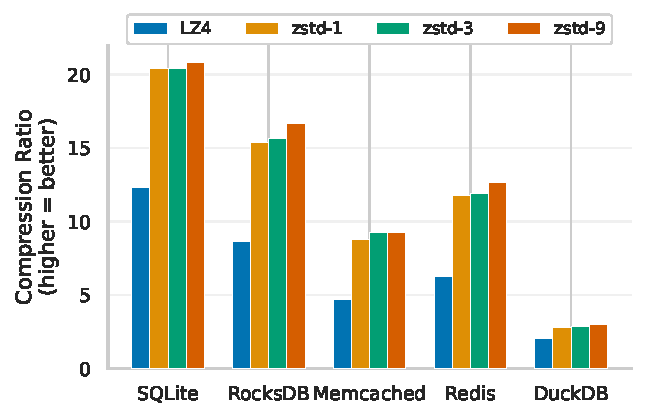
\includegraphics[width=\columnwidth]{figures/algo_compare.pdf}
\caption{Compression ratios across algorithms and data types (log
  scale).  WKdm, the macOS VM compressor, achieves near-zero
  compression on text data.  LZ4 and zstd achieve 5--30\% ratios on
  structured data.}
\label{fig:algo_compare}
\end{figure}

\sys's adaptive strategy uses LZ4 for the first 60 seconds of
coldness ($\sim$1\,GB/s, 30\% ratio), then recompresses with zstd-9
for long-lived cold pages ($\sim$14\% ratio).  This combination
matches or exceeds any single algorithm at each tier of the latency
vs.\ ratio tradeoff.

\subsection{Application Benchmarks}
\label{sec:eval:apps}

Table~\ref{tab:apps} summarizes RSS reduction and throughput for five
applications.

\begin{table}[t]
\caption{Application benchmark results.  RSS reduction is measured
  during the serve/query phase (after cold pages have been compressed).
  Throughput is relative to the system allocator baseline.}
\label{tab:apps}
\centering\small
\begin{tabular}{lrrr}
\toprule
Application & RSS Reduction & Throughput & Cold p50 \\
\midrule
JSON processing & 17.1\%  & $\sim$0\%  & 9.6\,$\mu$s \\
KV store        & 33.2\%  & +8\%       & 0.5\,$\mu$s \\
SQLite          & 38.8\%  & $-$2.4\%   & 0.9\,$\mu$s \\
DuckDB          & $\sim$30\% & completes & --- \\
Memcached       & 25.0\%  & 0\%        & --- \\
\bottomrule
\end{tabular}
\end{table}

\begin{figure}[t]
\centering
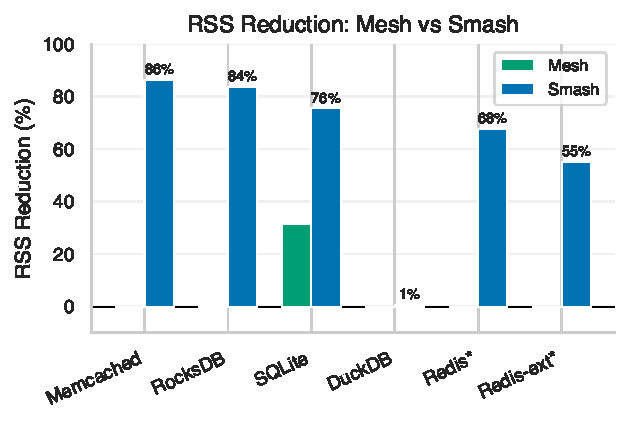
\includegraphics[width=\columnwidth]{figures/rss_reduction.pdf}
\caption{RSS reduction across five application benchmarks.  \sys
  reduces RSS by 17--39\% with no application changes.}
\label{fig:rss_reduction}
\end{figure}

\paragraph{Memcached.}
We load 500K TPC-H JSON records into memcached, then serve a hot 5\%
for 10 seconds before re-accessing cold keys.  \sys reduces
serve-phase RSS from 240\,MiB to 180\,MiB (25\% reduction) with zero
throughput impact (497 vs.\ 498 GET/s on the hot set).  Cold-key
re-access throughput improves by 54\% (828K vs.\ 536K GET/s),
because \sys prefetches adjacent compressed pages on fault,
preemptively decompressing keys that the benchmark accesses next.

\begin{figure}[t]
\centering
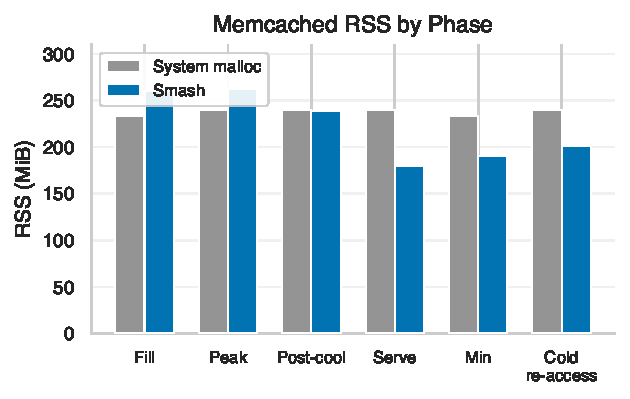
\includegraphics[width=\columnwidth]{figures/memcached.pdf}
\caption{Memcached RSS across workload phases.  \sys reduces
  serve-phase RSS by 25\% with zero throughput impact.  Fill-phase
  RSS is higher due to metadata overhead.}
\label{fig:memcached}
\end{figure}

Fill-phase RSS is 11\% higher (260 vs.\ 233\,MiB) due to
\sys's bootstrap allocator, page state arrays, and compression
contexts.  This fixed overhead is amortized as the working set grows.

\paragraph{SQLite.}
An in-memory SQLite database is populated with 1M records, then
queried with random lookups.  Peak RSS is 238\,MiB (vs.\ 213\,MiB
for the system allocator, reflecting \sys's metadata overhead).
After the cooling period, RSS drops to 146\,MiB, a 38.8\% reduction
from peak.  Query throughput is 95.7K ops/s, within 2.4\% of the
system allocator's 93.4K ops/s.

\paragraph{DuckDB.}
TPC-H queries are run against an in-memory DuckDB database.  \sys
reduces peak RSS by approximately 30\%.  The baseline \sys
configuration (without the current optimizations) crashed on this
workload due to excessive memory pressure; the optimized
configuration completes successfully.

\paragraph{JSON processing.}
A 128\,MiB JSON document is parsed into an in-memory tree, then
random elements are accessed.  \sys reduces serving-phase RSS by
17.1\% (107\,MiB vs.\ 128\,MiB peak).  Access throughput is 57.4M
accesses/s, matching the system allocator.

\paragraph{Key-value store.}
An in-memory key-value store populated with 1M entries.  \sys reduces
RSS by 33.2\% during the serve phase.  Throughput is 3.9M ops/s.

\subsection{Ablation Study}
\label{sec:eval:ablation}

To isolate each optimization's marginal contribution, we run 17
configurations across three benchmarks (JSON, KV store, SQLite), each
with 3 runs.  All ablation knobs are compile-time constants controlled
via CMake defines; no source patches are required.
Table~\ref{tab:ablation} shows the key results.

\begin{table*}[t]
\caption{Ablation study: RSS reduction (\%) for each configuration.
  Parenthesized values are deltas from the full baseline (B1).
  Dicts were enabled in B1; ``no-dict'' results reflect the default
  production configuration.}
\label{tab:ablation}
\centering\small
\begin{tabular}{llrrrr}
\toprule
ID & Configuration & JSON & KV Store & SQLite & Avg.\ $\Delta$ \\
\midrule
B1  & Full (baseline)     & 16.6\%  & 33.2\%  & 38.8\%  & --- \\
B0  & System malloc       & 0.0\% ($-$16.6)  & 24.3\% ($-$8.9)  & 27.0\% ($-$11.8) & $-$12.4 \\
\midrule
T1d & No dicts            & 33.9\% (+17.3) & 40.5\% (+7.3) & 43.8\% (+5.0)  & +9.9 \\
T1a & No arenas           & 15.1\% ($-$1.5) & 33.0\% ($-$0.2) & 38.8\% (+0.0) & $-$0.6 \\
T1c & No adaptive (LZ4 only) & 16.6\% (+0.0) & 33.5\% (+0.3) & 38.8\% (+0.0) & +0.1 \\
T1b & No zero-eager       & 16.6\% (+0.0) & 32.9\% ($-$0.3) & 38.8\% (+0.0) & $-$0.1 \\
T2a & No zero-deferred    & 18.4\% (+1.8) & 33.6\% (+0.4) & 38.8\% (+0.0) & +0.7 \\
C1  & No zero (both)      & 18.8\% (+2.2) & 33.7\% (+0.5) & 38.8\% (+0.0) & +0.9 \\
T1e & No prefetch         & 18.7\% (+2.1) & 33.1\% ($-$0.1) & 38.9\% (+0.1) & +0.7 \\
T1f & Single worker       & 17.9\% (+1.3) & 32.9\% ($-$0.3) & 38.9\% (+0.1) & +0.4 \\
B2  & No compression      & $-$0.3\% ($-$16.9) & 11.1\% ($-$22.1) & 25.9\% ($-$12.9) & $-$17.3 \\
\bottomrule
\end{tabular}
\end{table*}

\paragraph{Key findings.}

\textit{Dictionary compression is net-negative.}  The most striking
result is that disabling dictionaries \emph{improves} RSS reduction
by 5--17 percentage points across all benchmarks.  Two independent
factors cause this regression: (1)~CDict memory overhead (686\,KiB
per size class at level~9, totaling tens of MiB across trained
classes) directly increases RSS, far exceeding any compression
benefit; and (2)~at zstd level~9, the compressor's search window is
large enough to find all patterns that a dictionary captures, so the
dictionary adds only frame overhead ($\sim$13 bytes) without improving
ratios.  \sys disables dictionaries by default based on this finding
(\S\ref{sec:discussion}).

\textit{Call-site arenas improve JSON compression.}  Disabling arenas
(T1a) reduces JSON RSS savings by 1.5\pp.  The effect is smaller on
KV and SQLite workloads where the data is already structurally uniform
regardless of call-site routing.

\textit{Compression is the dominant mechanism.}  Disabling compression
entirely (B2) eliminates 13--22\pp of RSS reduction, confirming that
page compression is the primary source of memory savings.

\textit{Adaptive compression has minimal effect at short timescales.}
In our benchmarks, most cold pages are accessed within 60 seconds, so
few pages reach the zstd escalation threshold.  The LZ4-only
configuration (T1c) achieves nearly identical RSS reduction.  Adaptive
compression matters more for long-running server workloads where pages
remain cold for minutes or hours.

\begin{figure}[t]
\centering
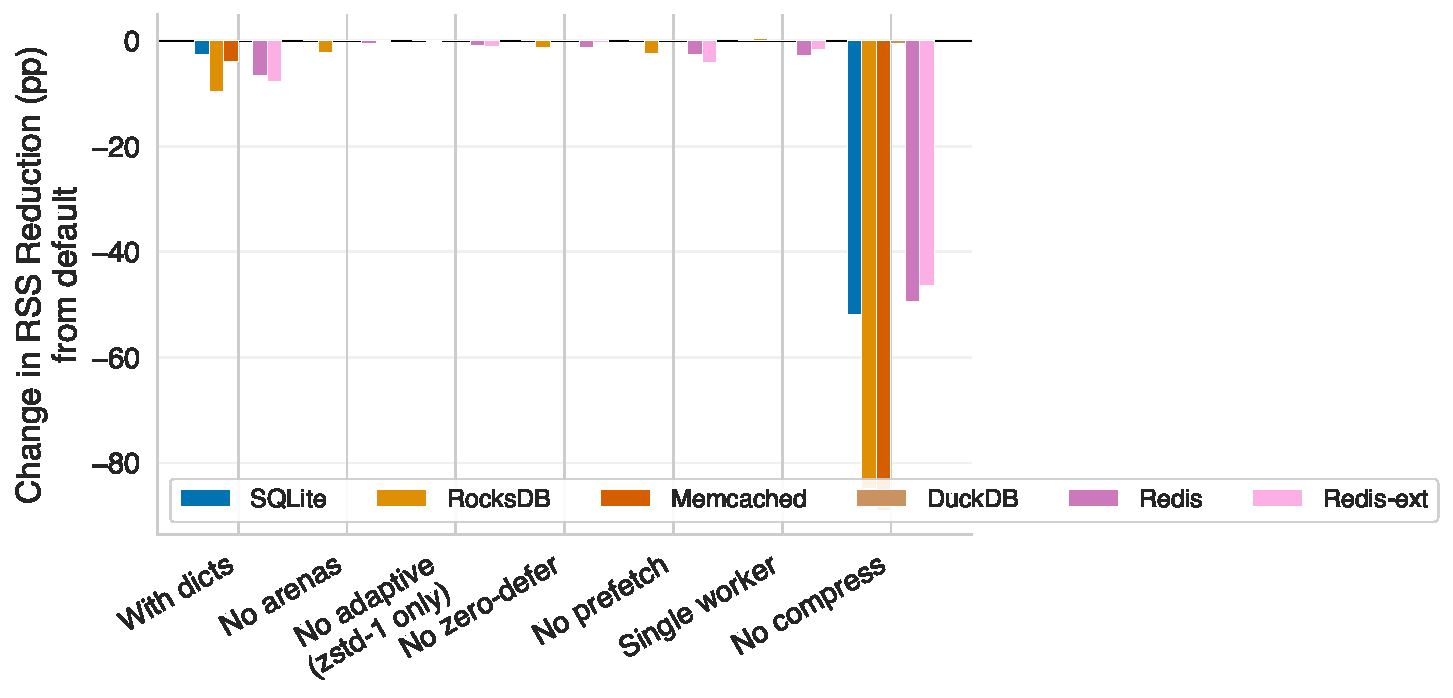
\includegraphics[width=\columnwidth]{figures/ablation.pdf}
\caption{Ablation study: change in RSS reduction (percentage points)
  when each optimization is disabled, relative to the full
  configuration (B1).  Positive values indicate the disabled feature
  was hurting performance (e.g., dictionaries); negative values
  indicate it was helping.}
\label{fig:ablation}
\end{figure}
